\documentclass[11pt,letterpaper]{article}
\usepackage[margin=0.85in]{geometry}
\usepackage[T1]{fontenc}
\usepackage[utf8]{inputenc}
\usepackage{lmodern,microtype,amsmath,amssymb,booktabs,array,xcolor}
\usepackage{tikz,pgfplots,listings,placeins}
\pgfplotsset{compat=1.18}
\usepackage[hidelinks]{hyperref}
\setlength{\parindent}{0pt}
\setlength{\parskip}{0.35em}
\setlength{\textfloatsep}{12pt}
\definecolor{inkblue}{RGB}{32,79,115}
\definecolor{warmred}{RGB}{179,69,56}
\newcommand{\pct}[1]{#1\%}
\lstset{language=Python,basicstyle=\ttfamily\footnotesize,
 keywordstyle=\color{inkblue},commentstyle=\color{gray},
 stringstyle=\color{warmred},breaklines=true,columns=fullflexible,
 keepspaces=true,showstringspaces=false,frame=single,rulecolor=\color{gray!35},
 backgroundcolor=\color{gray!4},aboveskip=7pt,belowskip=7pt,captionpos=b}
\definecolor{edaBlue}{HTML}{326A9A}
\definecolor{edaGreen}{HTML}{398570}
\definecolor{ratingOne}{HTML}{557FA3}
\definecolor{ratingTwo}{HTML}{86AEC4}
\definecolor{ratingThree}{HTML}{78A891}
\definecolor{ratingFour}{HTML}{335F50}
\title{Can Movies and Series' Descriptions Predict My Enjoyment\\Beyond Genre Labels?}
\author{CS156: Finding Patterns in Data with Machine Learning\\Pipeline 1}
\date{Fall 2026}
\begin{document}
\maketitle
\vspace{-1.4em}
\section{Introduction}
Hi Prof Watson. Since we are working on personal data for all three pipelines, I want to leave this course with a product I'll actually use. By the third pipeline, my goal is a project that helps me discover movies and series for my watchlist, then choose what to watch based on how I feel that evening. I imagine giving it clues such as ``the shrewdness of Wednesday Addams,'' ``a medieval setting like \emph{Merlin} or \emph{Legend of the Seeker},'' or ``rib-cracking comedy like Charlie Chaplin's \emph{The Great Dictator}.'' The hope is to find a title that fits that moment.

In my experience, a story is more enjoyable when it matches the mood I bring to it. This first assignment is supposed to build to that final goal by asking a narrower question before introducing context: \textbf{can movie and series descriptions predict my degree of enjoyment beyond what genre labels alone can predict?} Two titles labeled fantasy may emphasize different experiences, such as court intrigue and earnest adventure. A synopsis might preserve that distinction. Whether it helps predict \emph{my} taste requires a comparison, rather than an assumption that more text means more information of value.

I use four increasing liking levels, 1--4, with 4 highest. Level 1 does not necessarily mean dislike. A 0 means I haven't watched enough to rate a title and excludes it from modeling (more on that in data collection and preprocessing). A substantially watched but unfinished series receives a rating, reflecting the portion I have seen. The levels are ordered, but I have not established equal psychological distances between them.

\section{Data Collection}
\subsection{Data Sources}
My IMDb Watchlist is my primary data source because it’s a central hub where I add movies and series I'm watching or plan to watch, regardless of the streaming platform. However, some titles I've watched on the streaming platforms I use may not have made it to the watchlist. So, in addition to exporting my current watchlist as a CSV file, I also extract watch data from the various streaming platforms I use. For Netflix, Netflix provided a way to access my viewing-activity CSV through a \emph{Download} link on the web app\cite{netflix}. For HBO Max and Disney+, there's no dedicated view-activity section, so I scraped my in-app watch list data (again, this is possible because I usually add titles I'm watching or plan to watch to my platform-specific watchlist). So, I transcribed title, available year, and title-page URL from \href{https://play.hbomax.com/my-stuff}{HBO Max My List} and my \href{https://www.disneyplus.com/browse/watchlist}{Disney+ watchlist}. Saved lists capture my interest, whereas viewing activity records interactions. Neither indicates enjoyment or proves a title was finished, which is what I addressed when processing my data (in addition to structuring it for EDA and modeling).


\begin{table}[htbp]\centering\small
\begin{tabular}{@{}p{.27\linewidth}p{.20\linewidth}rp{.32\linewidth}@{}}\toprule
Source &Unit counted &Count &Meaning\\\midrule
Original IMDb CSV&Listed titles&302&Starting collection\\
HBO Max My List&Saved titles&36&Interest; possibly unwatched\\
Disney+ watchlist&Saved titles&30&Interest; possibly unwatched\\
Netflix CSV&Viewing events&622&Includes episodes\\
\bottomrule\end{tabular}
\caption{The four initial sources. A saved title or viewing event is not an enjoyment rating.}\label{tab:sources}\end{table}


\FloatBarrier
\section{Data Preprocessing}
\subsection{Observation Unit and Title Matching}
My observation is one movie or one whole series. Netflix's 134 \emph{Suits} events therefore become one preference example. Counting episodes separately would give that series disproportionate influence and could place closely related episodes in training and evaluation. A model could then recognize familiar characters or story language instead of generalizing to a new title, making its evaluation look more useful than it is for choosing something new to watch.

I removed explicit season/part/chapter suffixes while preserving the original strings and row numbers. A first-colon rule would damage \emph{Bad Boys: Ride or Die}. \emph{Money Heist: Part 1: Episode 3}, by contrast, explicitly identifies an episode. Ten \emph{The Hunting Party} variants required activity-page verification because their episode names lacked these markers. Ninety events had no series-name prefix; dates and episode numbers could not identify their parent reliably, so I preserved them as unresolved and excluded them from title matching. The 532 identifiable events became 27 distinct movie-or-series title candidates (not 27 episodes). Their IMDb identities were checked next.

\begin{lstlisting}[caption={Season, repeated-name and chapter rules preserve the parent title; a plain subtitle stays intact. Later rows are consolidated by that title.}]
marker = SEASON.match(title)
    if marker:
        return marker.group(1).strip()
    chunks = title.split(": ", 2)
    if len(chunks) == 3 and re.fullmatch(re.escape(chunks[0]) + r"\s+\d+", chunks[1], re.I):
        return chunks[0]
    chapter = CHAPTER.match(title)
    if chapter:
        return chapter.group(1).strip()
    return title  # Preserve film subtitles and ambiguous cases.

raw_netflix = pd.read_csv(ROOT / "data/raw/netflix_viewing_history_2026-10-17.csv")
parsed_netflix = raw_netflix.assign(canonical_candidate=raw_netflix.Title.map(title_candidate))
identified = parsed_netflix.loc[parsed_netflix.canonical_candidate.ne("")]
netflix_titles = identified.drop_duplicates("canonical_candidate")
\end{lstlisting}


The $36+30+27=93$ platform entries were compared with the original 302-row IMDb export locally. I normalized capitalization, accents, punctuation and spaces to look up possible title matches; an available year and film/series type rejected contradictions. A unique remaining candidate associated the platform row with an existing IMDb ID. Thus ``61 matches'' means 61 source rows mapped to 59 already-listed IMDb titles, with some titles appearing on multiple platforms. It does not mean 61 web requests or 61 newly discovered movies.

\begin{lstlisting}[caption={A local title-index lookup accepts one compatible IMDb candidate. Missing years remain missing; ambiguous or unmatched titles require review.}]
possible = name_index.get(normalize(row["title"]), set())
eligible = [key for key in possible
            if (not row["year"] or str(original_by_id[key]["Year"]) == row["year"])
            and compatible_type(row["type_hint"], original_by_id[key]["Title Type"])]
if len(eligible) == 1:
    initial_matches.append({**row,"record_id":eligible[0]})
\end{lstlisting}


I then reviewed the remaining 32 platform entries against title-page evidence. Only 31 added new IMDb IDs: Netflix's \href{https://www.imdb.com/title/tt11564570/}{\emph{Glass Onion: A Knives Out Mystery}} matched the shorter \emph{Glass Onion} already in my export. The other examples show why names alone were insufficient: Disney's \emph{Aladdin} needed the \href{https://www.imdb.com/title/tt6139732/}{2019 adaptation}, and HBO's \href{https://www.imdb.com/title/tt2975590/}{\emph{Batman v Superman: Dawn of Justice: Ultimate Edition}} was attached to the underlying 2016 film ID while retaining a note about the cut. The cut did not become another independent observation.

After these checks, I found which confirmed IDs were absent from my original IMDb list. I added the 17 missing HBO titles and 13 missing Disney+ titles to my IMDb watchlist, then exported it again: exactly 30 additions and no removals, giving 332 titles. One additional Netflix title, \href{https://www.imdb.com/title/tt14364480/}{\emph{Wake Up Dead Man}}, stayed outside that list and was retained separately in the combined table. I added my childhood classics \emph{Modern Times} (1936) and \emph{The Great Dictator} (1940), bringing the cross-source union to 335 distinct IMDb IDs. My final review removed the unseen 2011 \emph{Locke \& Key} pilot while retaining the 2020 series. Both \emph{Resident Evil} films (2002 and 2026) remain separate observations, each explicitly rated. Identical titles are therefore not automatically duplicates.

\begin{lstlisting}[caption={After reviewing identities, a set difference on IMDb IDs finds platform titles absent from the original list; source-level counts retain platform provenance.}]
new_ids = set(source_matches.record_id) - set(original_imdb.Const)
assert len(new_ids)==31
missing_by_source = (source_matches.loc[source_matches.record_id.isin(new_ids)]
                    .drop_duplicates(["source","record_id"]).groupby("source").size())
\end{lstlisting}

\begin{table}[htbp]\centering\small
\begin{tabular}{@{}p{.42\linewidth}p{.39\linewidth}r@{}}\toprule
Processing checkpoint &Unit counted &Count\\\midrule
Identifiable Netflix subset&Events $\rightarrow$ title candidates&$532\rightarrow27$\\
IMDb after HBO/Disney additions&Listed titles&332\\
IMDb after Chaplin additions&Listed titles&334\\
Cross-source union&Distinct IMDb IDs&335\\
After unseen-pilot exclusion&Titles for rating&334\\
Explicit rating 0&Insufficiently watched titles&130\\
Eligible rating 1--4&Modeling observations&204\\
\bottomrule\end{tabular}
\caption{Processing counts, separate from the four source counts. The Netflix-only title explains why the union exceeds the refreshed IMDb export.}\label{tab:processing}\end{table}


\FloatBarrier
\subsection{Explicit Ratings and Eligibility}
I exported the reconciled titles to an Excel rating sheet with title, year and stable IMDb ID so I could recognize adaptations. I filled it in Numbers, exported the completed document back to Excel, then read its \texttt{Ratings} worksheet with \texttt{read\_rating\_xlsx}. That helper reads the workbook's ZIP/XML cells, validates integer ratings and unique IDs, and preserves notes. A pandas \texttt{to\_csv} call turns the validated table into the CSV used for analysis. The two Chaplin ratings of 4 and the later instruction to retain both \emph{Resident Evil} films at 2 are recorded as explicit corrections, not guesses from viewing history.

\begin{lstlisting}[caption={The validated rating table is saved to CSV; zero-rated titles are excluded before a one-to-one metadata join.}]
replay_path = ROOT / "results/v2/ratings_replayed_from_excel.csv"
replay_path.parent.mkdir(parents=True,exist_ok=True)
label_table.to_csv(replay_path,index=False)

eligible_ratings = label_table.loc[label_table.rating.between(1,4)].copy()
model_data = eligible_ratings.merge(metadata,on=["record_id","title"],validate="one_to_one")
\end{lstlisting}


The completed ledger contains 204 ratings and 130 zeros. Zero means insufficient viewing to rate, not low enjoyment, so those rows are excluded before EDA or any vocabulary/classifier fitting. Only \texttt{genres} and \texttt{description\_text} are predictors; rating is the target. Title/ID, dates, viewing counts, platform membership, notes and correction history remain for checking the data.

\subsection{Synopsis and Genre Metadata}
IMDb's exported \texttt{Description} column was blank because it is a personal list-item note, not the plot summary \cite{imdblists}. I separately extracted the short plot-description container in the rendered IMDb watchlist, using title pages for the Netflix-only and Chaplin additions. I retained the exact text, IMDb ID and source URL, excluding surrounding credits, reviews, public scores and my account's stars from features.

Broad genres came from the refreshed IMDb CSV for every listed title. \emph{Wake Up Dead Man} was absent from that CSV because it was never added to the watchlist, \emph{not} because IMDb lacked its genre. I therefore read its \emph{Storyline Genres} on its IMDb title page. No Netflix genre replaced an IMDb genre. This title received 0 and is excluded from modeling, so all 204 modeled genre records use the same IMDb-export route.

For 37 rated titles, a platform supplied a name without a year, and that name matched only one title in my existing IMDb export. Those platform associations have less identity evidence than a title-and-year match: another adaptation could theoretically share the name. The IMDb records themselves still have a displayed title/year, a supplied rating, genres and a synopsis. Thus the uncertainty is about \emph{which platform entry refers to that record}, not 37 missing descriptions. These associations do not enter the model as features. All 204 eligible titles have complete metadata; no exact duplicate descriptions were found.

\FloatBarrier
\section{Exploratory Data Analysis}

The eligible sample has 204 titles: 150 movies, 51 series, two mini-series and one TV movie. The liking categories contain 45/72/56/31 titles. Their unequal support motivates a score that gives each category equal total importance. Descriptions contain 8--51 whitespace-delimited words (median 27), leaving limited recurring evidence for a specific story detail.

\begin{figure}[htbp]\centering
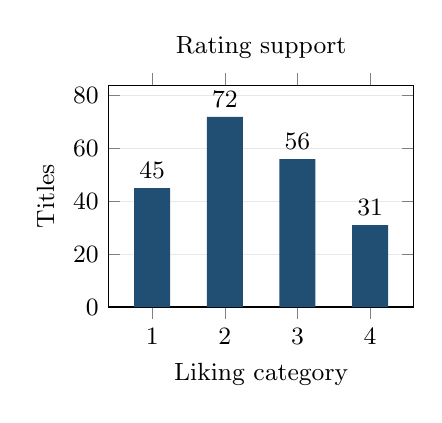
\begin{tikzpicture}
\begin{axis}[width=.45\linewidth,height=4.4cm,ybar,bar width=13pt,xmin=.4,xmax=4.6,ymin=0,ymax=84,xtick={1,2,3,4},xlabel={Liking category},ylabel={Titles},title={Rating support},font=\small,ymajorgrids=true,grid style={gray!18},nodes near coords]
\addplot[fill=inkblue,draw=none] coordinates {(1,45.000000) (2,72.000000) (3,56.000000) (4,31.000000)};
\end{axis}\end{tikzpicture}
\hfill
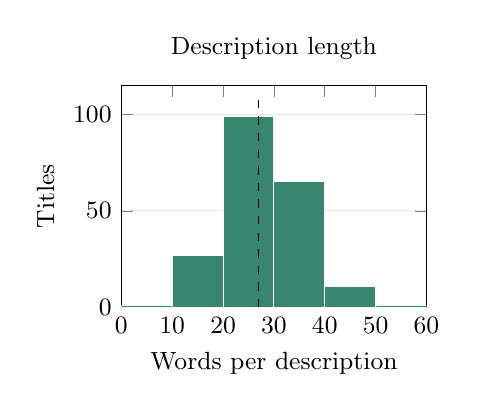
\begin{tikzpicture}
\begin{axis}[width=.45\linewidth,height=4.4cm,xmin=0,xmax=60,ymin=0,ymax=115,xtick={0,10,20,30,40,50,60},xlabel={Words per description},ylabel={Titles},title={Description length},font=\small,ymajorgrids=true,grid style={gray!18}]
\addplot[ybar interval,fill=edaGreen,draw=white] coordinates {(0,1.000000) (10,27.000000) (20,99.000000) (30,65.000000) (40,11.000000) (50,1.000000) (60,0.000000)};
\draw[dashed] (axis cs:27,0)--(axis cs:27,110);
\end{axis}\end{tikzpicture}
\caption{Eligible labels and description lengths; the dashed line marks the median. Zeros are excluded.}\label{fig:eda}\end{figure}

193 titles have several genres; 17 labels form 105 observed combinations. Choosing just one genre would discard labels, while treating every combination as a new category would fragment this small sample. I retain the individual indicators. The overlapping groups below contain all four liking levels; broad genre is not itself an enjoyment label.

\begin{figure}[htbp]\centering
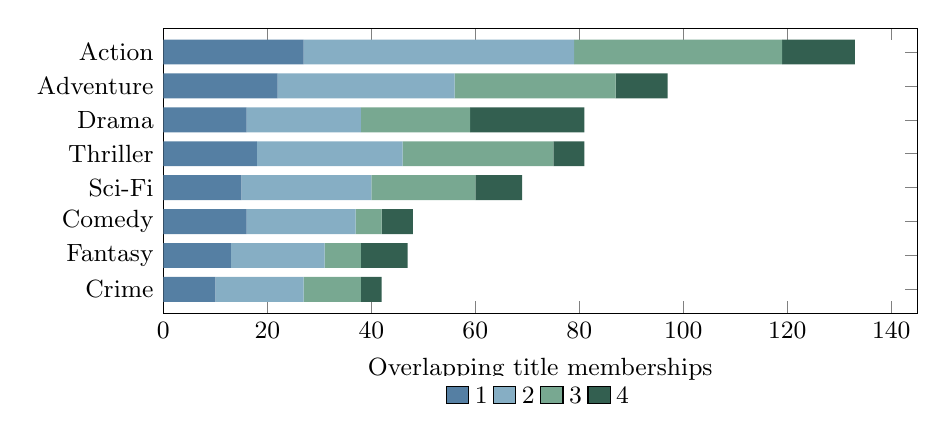
\begin{tikzpicture}
\begin{axis}[width=.92\linewidth,height=5.2cm,xbar stacked,bar width=9pt,xmin=0,xmax=145,symbolic y coords={Action,Adventure,Drama,Thriller,Sci-Fi,Comedy,Fantasy,Crime},ytick=data,y dir=reverse,xlabel={Overlapping title memberships},font=\small,legend style={at={(.5,-.22)},anchor=north,legend columns=4,draw=none}]
\addplot[fill=ratingOne,draw=none] coordinates {(27,Action) (22,Adventure) (16,Drama) (18,Thriller) (15,Sci-Fi) (16,Comedy) (13,Fantasy) (10,Crime)};
\addplot[fill=ratingTwo,draw=none] coordinates {(52,Action) (34,Adventure) (22,Drama) (28,Thriller) (25,Sci-Fi) (21,Comedy) (18,Fantasy) (17,Crime)};
\addplot[fill=ratingThree,draw=none] coordinates {(40,Action) (31,Adventure) (21,Drama) (29,Thriller) (20,Sci-Fi) (5,Comedy) (7,Fantasy) (11,Crime)};
\addplot[fill=ratingFour,draw=none] coordinates {(14,Action) (10,Adventure) (22,Drama) (6,Thriller) (9,Sci-Fi) (6,Comedy) (9,Fantasy) (4,Crime)};
\legend{1,2,3,4}
\end{axis}\end{tikzpicture}
\caption{Eight most represented genres, split by liking category. Memberships overlap and must not be added as independent observations.}\label{fig:genres}\end{figure}

\begin{lstlisting}[caption={Multi-genre labels are expanded only to summarize membership. the modeling table retains one row per title.}]
genre_support = (
    data.assign(genre=data.genres.str.split(",")).explode("genre")
        .assign(genre=lambda frame: frame.genre.str.strip())
        .groupby("genre").size().sort_values(ascending=False).rename("eligible_titles")
)
display(genre_support.to_frame())
\end{lstlisting}


\FloatBarrier
\section{Feature Engineering}
The cleaned table still contains text, labels and audit columns. Before learning any representation, I assign title IDs to training and held-out partitions. Within each training partition, a pipeline learns genre columns, word vocabulary and inverse document frequencies; it only \emph{transforms} the held-out titles with those fitted rules. Inner validation repeats this separation. Otherwise, an evaluation description could influence which words the model knows, giving information that would be unavailable for a genuinely new title.

The inputs are the two columns \texttt{genres} and \texttt{description\_text}. \texttt{rating} is kept separately as the target. There are no missing eligible predictors to impute, and platform/year/viewing counts are not numeric features to scale. I encode the multi-valued genre category and rescale the resulting feature vectors. This is where category encoding and scaling enter this particular dataset.

\subsection{Genre Encoding and Normalization}
A genre vector $g$ contains a 1 for each label present and 0 otherwise. With $k$ labels its Euclidean length is $\lVert g\rVert_2=\sqrt{\sum_jg_j^2}=\sqrt{k}$. I use
\[
\tilde g=\frac{g}{\lVert g\rVert_2}.
\]
For Comedy/Drama/War, the three nonzero entries become $(1,1,1)/\sqrt3=(0.577,0.577,0.577)$. The result has length 1, just like a one-tag title: having more tags no longer automatically creates a larger input. The tradeoff is that each individual tag becomes weaker when more are present. Label count is still recoverable from the nonzero pattern; normalization controls magnitude rather than erasing that information.

\subsection{TF-IDF Descriptions}
A word repeated within a synopsis may characterize it, but a word appearing in almost every synopsis distinguishes little. Term frequency (TF) counts within-description occurrences; inverse document frequency (IDF) weights those counts by rarity across \emph{training} descriptions. With $m$ training titles, count $c_{dt}$ for word $t$ in description $d$, and $\mathrm{df}_t$ training descriptions containing it,
\[
\mathrm{idf}_t=1+\log\frac{1+m}{1+\mathrm{df}_t},\qquad
u_{dt}=c_{dt}\,\mathrm{idf}_t,\qquad
\tilde u_d=\frac{u_d}{\lVert u_d\rVert_2}.
\]
The logarithm compresses the rarity ratio so one unusual word does not receive an enormous multiplier. Adding 1 in the ratio smooths small counts and avoids zero denominators; the final $+1$ leaves an everywhere-present word with weight 1 instead of deleting it. For illustration, with 163 training descriptions, words in two versus 81 titles get IDFs about 5.00 versus 1.69. This is rarity, not liking: the classifier must learn the rating association.

I lowercase single words, require appearance in at least two training titles and cap vocabulary at 3,000. The minimum frequency reduces singleton parameters that cannot be checked against another training title; the cap is a fixed computational safeguard, not a tuned claim of optimality. I retain common words and negation rather than applying a blanket stop-word list. Word order and much of a story's tone are lost, a limitation that matters for the eventual ``vibe'' goal.

Text vectors are normalized so repeating or lengthening a synopsis does not automatically enlarge its input. Joining two unit-length blocks gives length $\sqrt2$, so the combined input is
\[
x=\frac{[\tilde g,\tilde u]}{\lVert[\tilde g,\tilde u]\rVert_2}.
\]
When both blocks are nonzero, each is divided by $\sqrt2$; the example's genre values become $1/\sqrt6=0.408$. This fixes equal initial block magnitude, not equal predictive usefulness. An all-zero block stays zero. Input normalization controls scale; regularization below controls learned weights. The notebook independently reconstructs TF-IDF from counts and verifies equality with the library vectorizer \cite{sklearntext}.

\section{Model Selection}
\subsection{Prediction Task and Controlled Comparison}
I predict one of four liking categories. Squared-error regression would impose equal numerical gaps and require interpreting a value such as 2.6, neither of which my labels establish. Nominal classification avoids that distance assumption but does not use the ordering during training. An ordinal model can preserve order without equal spacing. I opted against it as my starting choice because I wanted a transparent class-by-class reference; a simple proportional-odds model would additionally share feature effects across ordered thresholds, an assumption I have not established. This is a bounded starting choice, not evidence that ordinal methods are inferior.

The first comparison holds the learning rule fixed and changes only the information supplied: genres, descriptions, or both. A training-fold majority-label rule is the reference without story information. Each learned condition validates the same three $C$ values on identical inner partitions, refits its selected value, then predicts the same outer held-out titles. This pairing asks whether extra text helps this learner rather than whether one model happened to see easier test movies. Text alone measures its standalone value; \emph{combined minus genres} answers the research question.

Regularized multinomial logistic regression is my reference because an additive genre/word score is inspectable and shrinkage limits large weights supported by few titles. The training sets have only 163--164 titles and hundreds of word features. I reuse the score/likelihood/gradient pattern from Class Session 6 and explicit updates from Sessions 7--8, adapting binary examples to four classes. Library tools still handle tokenization, sparse matrices and splitting \cite{course}.

\subsection{Logistic Learning}
For class $k$, coefficients $w_k$ add feature contributions and intercept $b_k$ provides a class offset:
\[
z_k=w_k^\top x+b_k,\qquad
p_k=\frac{e^{z_k}}{\sum_{j=1}^{4}e^{z_j}},\qquad
\hat y=\arg\max_k p_k.
\]
Scores can be negative and need not sum to one. Exponentiation makes them positive while preserving order; division by the sum produces four outputs totaling one. Equal scores give 25\% each. Only differences matter: $p_a/p_b=e^{z_a-z_b}$. Subtracting the largest score before exponentiating leaves these ratios unchanged and prevents numerical overflow.

\begin{lstlisting}[caption={The manual forward pass converts relative class scores into stable softmax outputs.}]
def softmax(scores):
    shifted=scores-np.max(scores,axis=1,keepdims=True)
    numerator=np.exp(shifted)
    return numerator/numerator.sum(axis=1,keepdims=True)
\end{lstlisting}


Fitting should reward probability on the recorded category. Negative log probability provides a smooth cost: a true-category output of 0.8 costs $-\log(0.8)=0.223$, while 0.01 costs 4.605. Thus confidently wrong predictions are expensive. For training counts $n_k$, give each title weight $s_i=n/(4n_{y_i})$. Each category then contributes total weight $n_k\,n/(4n_k)=n/4$, so common rating 2 does not dominate the loss. These counts are recomputed inside training folds.

With $S=\sum_i s_i=n$, the objective is
\[
J(W,b)=-\frac1S\sum_i s_i\log p_{i,y_i}+\frac{\lVert W\rVert_F^2}{2SC}.
\]
The first term averages prediction cost. The second sums squared coefficients: magnitude 4 costs sixteen times magnitude 1, discouraging extreme responses to scarce evidence. $C$ controls the tradeoff; smaller $C$ increases this penalty. The intercept is unpenalized. Balancing log loss encourages equal-category attention, but does not directly optimize balanced accuracy, which scores hard decisions.

Let $Y$ contain a 1 at each true class and 0 elsewhere, and $P$ contain predicted probabilities. Rows of $X$ are titles and columns are features; rows of $W$ hold class coefficients. The residual $P-Y$ measures probability error: subtracting 1 in the true class pushes its score up during a negative-gradient update; other class scores are pushed down. Weighting by $s_i/S$, multiplying by each title's features, and adding the L2 derivative gives
\[
R_{ik}=\frac{s_i}{S}(P_{ik}-Y_{ik}),\qquad
\nabla_WJ=R^\top X+\frac{W}{SC},\qquad \nabla_bJ=\sum_iR_i.
\]
The penalty derivative pulls coefficients toward zero. Collecting $W$ and $b$ into parameter vector $\theta$, my code uses step size $\eta$ and updates as $\theta_{\mathrm{new}}=\theta-\eta\nabla J$: a positive derivative means reducing that parameter lowers the local loss. It estimates a step size from recent parameter/gradient changes, then halves any step that fails to reduce the loss sufficiently. It stops when the largest absolute gradient is at most $10^{-6}$, with a 2,000-update cap and convergence failures treated as errors. This owns the learning updates rather than calling a library's logistic fitter.

\begin{lstlisting}[caption={The handwritten backward pass turns class-probability errors into coefficient and intercept gradients; the full learner applies and checks its own updates.}]
residual=softmax(scores)
residual[np.arange(len(encoded_y)),encoded_y]-=1
residual*=sample_weights[:,None]/S
grad_W=np.asarray(X.T@residual).T+W/(S*C)
grad_b=residual.sum(axis=0)
\end{lstlisting}


Finite-difference checks perturb parameters and compare the numerical loss change with these derivatives. Dense and sparse calculations agree, and small synthetic fits match an independent scikit-learn logistic reference. These are implementation checks, not evidence of movie-prediction quality. The notebook also records the actual optimization-loss trace for the held-out worked example.

\subsection{Alternative Classifiers and Parameters}
To test whether the answer depends on that learning rule, I compare four motivated families, three settings each (Table~\ref{tab:menu}). Genres and combined features each receive the twelve configurations, identical development partitions and the same selection score. Equal search counts control the budget, although the parameters do not define identical capacity scales.

\begin{table}[htbp]\centering\small
\begin{tabular}{@{}p{.21\linewidth}p{.23\linewidth}p{.49\linewidth}@{}}\toprule
Classifier &Settings &Motivation\\\midrule
Manual logistic&$C=0.1,1,10$&Additive class scores; coefficient shrinkage\\
Linear SVM&$C=0.1,1,10$&Sparse linear decisions with a margin-based loss\\
Complement NB&$\alpha=10,1,0.1$&Smoothed feature evidence from other categories\\
Decision tree&Depth $2,4,8$&Threshold rules and feature interactions; at least five titles per leaf\\
\bottomrule\end{tabular}
\caption{Four families, twelve configurations per feature condition. Logistic/SVM/tree use balanced training-fold class weights; NB uses its native complement estimates.}\label{tab:menu}\end{table}


\textbf{Linear SVM.} Four one-versus-rest problems each separate one rating from the others. For $r=+1$ in the selected class and $r=-1$ otherwise, and linear score $f$, squared-hinge loss is $[\max(0,1-rf)]^2$. A positive title scored 0.2 costs 0.64, scored 1.2 costs zero, and scored $-0.2$ costs 1.44. Correct sign alone is insufficient: the model seeks a safety margin. L2 controls coefficient growth, while $C$ trades shrinkage against this loss. The largest of four scores chooses the rating; no probability calibration is implied. Comparing it with logistic tests a different sparse linear learning rule \cite{svm}.

\textbf{Complement Naive Bayes.} Let $A_{kj}=\sum_{i:y_i\ne k}x_{ij}$ be feature $j$'s mass among all \emph{other} rating categories. With $p$ input features,
\[
\bar\theta_{kj}=\frac{A_{kj}+\alpha}{\sum_\ell A_{k\ell}+\alpha p},\qquad
s_k(x)=-\sum_jx_j\log\bar\theta_{kj}.
\]
A title poorly explained by category $k$'s complement receives a high score for $k$. Adding $\alpha$ prevents zero proportions and infinite log penalties; more smoothing moves estimates toward uniformity, stabilizing rare evidence but possibly washing out distinctions. Logs turn multiplicative feature evidence into a manageable sum. Here feature weights supply fractional mass rather than literal counts. This native \texttt{norm=False} rule is a contrasting text-oriented approximation, not a model of narrative order or correlated meaning \cite{cnb}.

\textbf{Decision tree.} A path asks successive feature-threshold questions, allowing one genre or word to matter differently after another branch. If $q_k$ is a node's weighted class fraction, Gini impurity is $G=1-\sum_kq_k^2$: two draws match categories with probability $\sum_kq_k^2$, so $G$ measures their chance of differing. It is 0 for a pure node and 0.75 for four equal classes. A split maximizes the drop from parent impurity to the child impurities averaged by child weight. Weighting matters because a tiny pure child should not overshadow a large mixed one. This greedy rule finds a useful immediate split, not a globally optimal tree. Depth limits and a five-title minimum leaf constrain unstable rules on sparse features \cite{tree}.

For each family, development scores choose its setting and then the overall winner among the twelve configurations. Exact ties favor logistic, SVM, NB, then tree; within a family they favor smaller $C$, larger $\alpha$, or shallower depth. Test scores never change these choices. A selected development maximum can be optimistic, which is why the final assessment uses held-out predictions.

\begin{lstlisting}[caption={Five-fold development selection fits the complete feature-and-classifier pipeline. Family finalists are explicitly refitted afterward; the test set does not select them.}]
search = GridSearchCV(
    candidate_pipeline, parameter_grid,
    scoring="balanced_accuracy", cv=inner_splits,
    refit=False, n_jobs=1, error_score="raise",
)
search.fit(X_dev, y_dev)
\end{lstlisting}


\FloatBarrier
\section{Evaluation}
\subsection{Nested Cross-Validation}
With 204 rated titles, one 20\% test would contain only about six highest-liking examples. Instead, five outer folds give every title one held-out prediction; three repetitions (seeds 156, 1156, 2156) show sensitivity to splitting. Stratification keeps all four categories represented. Each outer fit uses 163--164 titles. Three inner folds select $C\in\{0.1,1,10\}$ from training data, then the selected pipeline refits on the outer training set. The outer labels assess that complete procedure rather than choosing its setting \cite{nested}.

Titles are distinct, but related films and series can still share language. A separate conservative franchise map holds related-work groups apart at both CV levels. That asks a harder, somewhat different question about unseen groups, so its score difference is a sensitivity check rather than a causal estimate of leakage. Repeated folds also share training titles; their ranges are not independent confidence intervals \cite{bates}.

\subsection{A Score for This Question}
I want success across all four liking categories, not mainly rating 2. Balanced accuracy (BA) calculates each category's recall, then averages:
\[
\mathrm{BA}=\frac14\sum_{k=1}^4
\frac{\#\{i:y_i=k,\hat y_i=k\}}{\#\{i:y_i=k\}}.
\]
Imagine first selecting a liking category uniformly, then selecting a title within it. BA is the chance of recognizing that title's rating under this equal-category sampling rule. The 31 highest-liking examples therefore have the same total score weight as the 72 rating-2 examples. Always predicting 2 gives BA 25\%, despite ordinary accuracy of $72/204=35.29\%$. One additional correct rating-4 prediction changes pooled BA by $1/(4\times31)=0.81$ percentage points, versus 0.35 points for rating 2.

BA does not distinguish neighboring from extreme errors, so ordered confusion matrices show that missing context. I do not add F1/AUC simply because they exist: they answer other weighting/ranking questions. For each repetition, I pool all 204 held-out predictions and subtract genre BA from combined BA. This paired difference is the research contrast; its three-repeat range describes split sensitivity.

\begin{lstlisting}[caption={Manual balanced recall averages success within the four true categories; the notebook checks all pooled primary scores against this calculation.}]
def balanced_recall(y_true,y_pred):
    recalls=[]
    for level in [1,2,3,4]:
        in_class=np.asarray(y_true)==level
        recalls.append(np.mean(np.asarray(y_pred)[in_class]==level))
    return float(np.mean(recalls))
\end{lstlisting}


\subsection{Validation Strategy and Data Budget}
The classifier-family comparison uses a common 41-title outer test per seed, with 163 development titles. Five-fold development selection fits each candidate on 130--131 titles, validating 32--33 at a time; every development title validates once. A single validation split fits on 130 and validates on 33. Both strategies then refit each family's selected setting on all 163 development titles before the common test. This matches final training size rather than confusing a CV advantage with access to more final training examples.

\begin{table}[htbp]\centering\small
\begin{tabular}{@{}p{.31\linewidth}p{.23\linewidth}p{.20\linewidth}r@{}}\toprule
Procedure &Candidate training &Validation coverage &Final fit / test\\\midrule
Five-fold selection, refit&130--131 per fold&163&$163/41$\\
Single validation, refit&130&33&$163/41$\\
Single validation, cached fit&130&Same 33&$130/41$\\
\bottomrule\end{tabular}
\caption{The single three-way split is 130/33/41 (about 64/16/20). Refitting creates the final 80/20 development/test comparison.}\label{tab:allocation}\end{table}


The cached 130-title fit holds the single-selected family and setting fixed; its comparison with the 163-title refit illustrates the cost of leaving validation titles unused after selection. Vocabulary and class weights also change, so this is a practical data-budget contrast rather than a pure causal effect of sample count. A plain train/test split could assess a procedure fixed beforehand, but could not also select twelve settings using the same test.

The family comparison uses $12\times5=60$ CV candidate fits, 12 single-validation fits and eight family-finalist refits per seed/feature condition: $80\times3\times2=480$ successful comparison fits. Cached fits add no extra training. All family choices are saved before test scoring. This is an exploratory personal archive whose earlier draft results were already reviewed; the revised protocol fixes choices and partitions before its evaluation runs, but reused titles are not fresh confirmatory evidence. Small data makes the computation affordable, not the uncertainty negligible.

\FloatBarrier
\section{Results}
\subsection{Do Descriptions Add to Genres?}

\begin{table}[htbp]\centering\small
\begin{tabular}{@{}lrr@{}}\toprule
Information supplied &Mean BA (\%) &Three-repeat range (\%)\\\midrule
Majority&25.00&25.00--25.00\\
Genres&33.62&31.77--35.73\\
TF-IDF descriptions&26.31&24.05--27.70\\
Genres + TF-IDF&34.16&29.76--39.29\\
\bottomrule\end{tabular}
\caption{Paired nested-CV results for the same 204 eligible titles. Ranges are descriptive, not confidence intervals.}\label{tab:primary}\end{table}

Descriptions increase mean BA from 33.62\% to 34.16\%, only \textbf{+0.53 percentage points}. The three changes are $+0.04$, $+3.57$, $-2.01$ pp. Thus the combined representation is slightly better on average under this learner, but the gain is small and changes sign. Text alone averages 26.31\%, near the constant-category reference; these short word vectors are not yet a dependable representation of my taste.

\begin{figure}[htbp]\centering
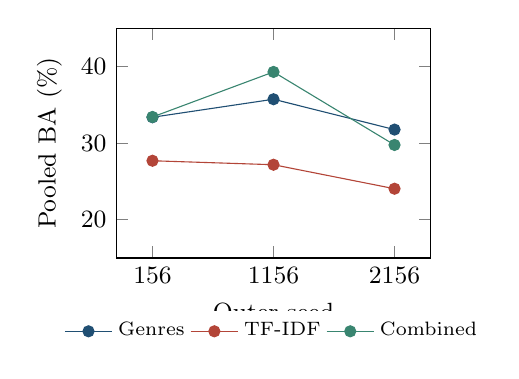
\begin{tikzpicture}
\begin{axis}[width=.46\linewidth,height=4.5cm,xmin=.7,xmax=3.3,ymin=15,ymax=45,xtick={1,2,3},xticklabels={156,1156,2156},xlabel={Outer seed},ylabel={Pooled BA (\%)},font=\small,legend style={at={(.5,-.23)},anchor=north,legend columns=3,draw=none,font=\scriptsize}]
\addplot[inkblue,mark=*] coordinates {(1,33.376536) (2,35.729327) (3,31.766513)};
\addplot[warmred,mark=*] coordinates {(1,27.698733) (2,27.179980) (3,24.046339)};
\addplot[edaGreen,mark=*] coordinates {(1,33.413338) (2,39.294995) (3,29.760945)};
\legend{Genres,TF-IDF,Combined}
\end{axis}\end{tikzpicture}
\hfill
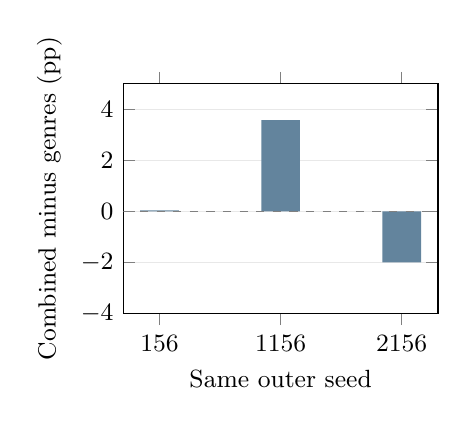
\begin{tikzpicture}
\begin{axis}[width=.46\linewidth,height=4.5cm,ybar,bar width=14pt,xmin=.7,xmax=3.3,ymin=-4,ymax=5,xtick={1,2,3},xticklabels={156,1156,2156},xlabel={Same outer seed},ylabel={Combined minus genres (pp)},font=\small,ymajorgrids=true,grid style={gray!18}]
\addplot[fill=inkblue!70,draw=none] coordinates {(1,0.036802) (2,3.565668) (3,-2.005568)};\draw[dashed,gray] (axis cs:.7,0)--(axis cs:3.3,0);
\end{axis}\end{tikzpicture}
\caption{The same held-out titles support both absolute-score and incremental comparisons. Changing the partition can reverse the text benefit.}\label{fig:primary}\end{figure}


\subsection{Which Classifiers Survive Validation?}

\begin{table}[htbp]\centering\small
\begin{tabular}{@{}lrrr@{}}\toprule
Combined-feature family &CV dev. BA (\%) &CV test BA (\%) &Single-val. test BA (\%)\\\midrule
Logistic&34.31&34.66&34.03\\
Linear SVM&32.45&33.09&33.49\\
Complement NB&28.25&27.10&24.03\\
Tree&27.20&29.35&27.10\\
\bottomrule\end{tabular}
\caption{Development columns average each family's selected setting over three seeds; they are optimistic tuning summaries. Both test procedures refit on 163 titles.}\label{tab:families}\end{table}

\begin{figure}[htbp]\centering
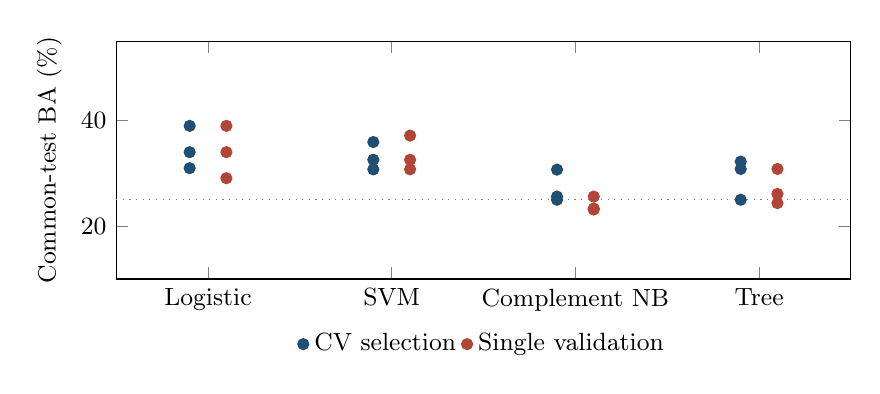
\begin{tikzpicture}
\begin{axis}[width=.9\linewidth,height=4.6cm,xmin=.5,xmax=4.5,ymin=10,ymax=55,xtick={1,2,3,4},xticklabels={Logistic,SVM,Complement NB,Tree},ylabel={Common-test BA (\%)},font=\small,legend style={at={(.5,-.18)},anchor=north,legend columns=2,draw=none}]
\addplot[only marks,mark=*,color=inkblue] coordinates {(0.9,38.989899) (0.9,34.015152) (0.9,30.984848) (1.9,35.934343) (1.9,32.575758) (1.9,30.757576) (2.9,25.000000) (2.9,25.606061) (2.9,30.707071) (3.9,25.000000) (3.9,32.222222) (3.9,30.833333)};
\addlegendentry{CV selection}
\addplot[only marks,mark=*,color=warmred] coordinates {(1.1,38.989899) (1.1,34.015152) (1.1,29.090909) (2.1,37.146465) (2.1,32.575758) (2.1,30.757576) (3.1,23.156566) (3.1,25.606061) (3.1,23.333333) (4.1,24.368687) (4.1,26.111111) (4.1,30.833333)};
\addlegendentry{Single validation}
\draw[dotted,gray] (axis cs:.5,25)--(axis cs:4.5,25);
\end{axis}\end{tikzpicture}
\caption{Each dot is a development-tuned family evaluated on one shared test partition; the dotted majority reference is 25\%. A high test point does not retroactively choose the family.}\label{fig:families}\end{figure}

\begin{table}[htbp]\centering\small
\begin{tabular}{@{}rllrr@{}}\toprule
Seed &Selector &Development winner &Dev. BA (\%) &Test BA (\%)\\\midrule
156&CV&Logistic ($C=10.0$)&34.45&38.99\\
156&Single validation&Linear SVM ($C=10.0$)&26.63&37.15\\
1156&CV&Logistic ($C=0.1$)&33.15&34.02\\
1156&Single validation&Logistic ($C=0.1$)&38.81&34.02\\
2156&CV&Logistic ($C=0.1$)&35.33&30.98\\
2156&Single validation&Logistic ($C=1.0$)&42.28&29.09\\
\bottomrule\end{tabular}
\caption{The actual family choices before test assessment. Keeping the winner even when another family tests better measures the selection procedure honestly.}\label{tab:winners}\end{table}

The tree offers interactions, but its CV-tuned combined test scores range from 25.00\% to 32.22\%. That spread shows why a plausible model needs held-out evidence, not just an appealing mechanism. Linear families and complement statistics also vary with selection strategy; these three small tests do not establish a permanent best algorithm. All three CV selectors chose logistic regression with combined features, supporting it within this limited candidate menu. Single validation chose SVM once and logistic twice. The table retains those choices even when another family tests better.


\subsection{CV, Single Validation and Training Size}

\begin{table}[htbp]\centering\small
\begin{tabular}{@{}lrrr@{}}\toprule
Selector / training titles &Genres BA (\%) &Combined BA (\%) &Change (pp)\\\midrule
CV / 163&32.53&34.66&+2.13\\
Single validation / 163&29.10&33.42&+4.32\\
Single validation / 130&36.29&33.83&-2.46\\
\bottomrule\end{tabular}
\caption{Mean common-test scores for overall development-selected procedures. Genre and combined winners can be different families, so this contrast includes the selection rule.}\label{tab:strategy}\end{table}

\begin{figure}[htbp]\centering
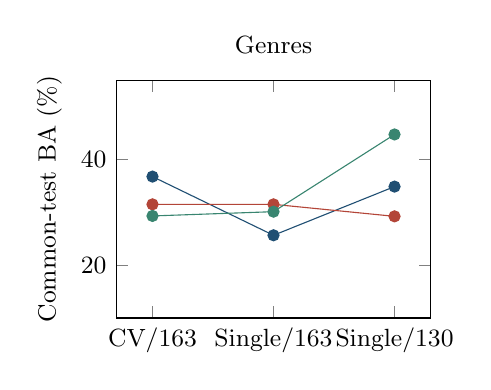
\begin{tikzpicture}
\begin{axis}[width=.46\linewidth,height=4.6cm,xmin=.7,xmax=3.3,ymin=10,ymax=55,xtick={1,2,3},xticklabels={CV/163,Single/163,Single/130},title={Genres},ylabel={Common-test BA (\%)},font=\small,legend style={at={(.5,-.22)},anchor=north,legend columns=3,draw=none,font=\scriptsize}]
\addplot[inkblue,mark=*] coordinates {(1,36.767677) (2,25.656566) (3,34.873737)};
\addplot[warmred,mark=*] coordinates {(1,31.515152) (2,31.515152) (3,29.242424)};
\addplot[edaGreen,mark=*] coordinates {(1,29.318182) (2,30.126263) (3,44.747475)};

\end{axis}\end{tikzpicture}
\hfill
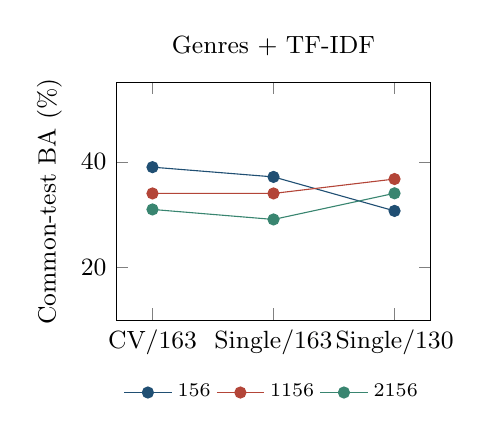
\begin{tikzpicture}
\begin{axis}[width=.46\linewidth,height=4.6cm,xmin=.7,xmax=3.3,ymin=10,ymax=55,xtick={1,2,3},xticklabels={CV/163,Single/163,Single/130},title={Genres + TF-IDF},ylabel={Common-test BA (\%)},font=\small,legend style={at={(.5,-.22)},anchor=north,legend columns=3,draw=none,font=\scriptsize}]
\addplot[inkblue,mark=*] coordinates {(1,38.989899) (2,37.146465) (3,30.707071)};
\addplot[warmred,mark=*] coordinates {(1,34.015152) (2,34.015152) (3,36.742424)};
\addplot[edaGreen,mark=*] coordinates {(1,30.984848) (2,29.090909) (3,34.040404)};
\legend{156,1156,2156}
\end{axis}\end{tikzpicture}
\caption{Colors follow the same outer seed. First compare selectors with equal final training size; then compare the single-selected setting with and without refitting on validation titles.}\label{fig:strategy}\end{figure}

For the selected combined procedure, CV averages 34.66\% versus 33.42\% for single validation. CV is higher here, but this is not a general ranking of split methods. Each test has only six rating-4 titles; one extra success there moves BA by 4.17 points. The three tests also overlap, and development maxima are noisy after searching twelve settings. CV broadens the selection evidence without manufacturing new ratings.

Refitting the single-selected combined settings on 163 instead of 130 titles changes mean BA from 33.83\% to 33.42\% (-0.41 pp), with per-seed changes $+6.44$, $-2.73$, $-4.95$ pp. Family and setting stay fixed in this contrast; learned vocabulary and weights can change. A larger training budget therefore has an observable but split-sensitive consequence, rather than a guaranteed improvement.


\FloatBarrier
\section{Model Diagnostics}
\subsection{Ordered Errors}

On seed 156, text corrects 18 genre errors and introduces 16 new ones. Correct totals rise from 65 to 67, but BA rises by only 0.04 pp. The category mix explains why: correct counts change by $+0$, $+5$, $-2$, $-1$ across ratings 1--4. A gain on common rating 2 can be offset by fewer successes on rare rating 4.

\begin{figure}[htbp]\centering
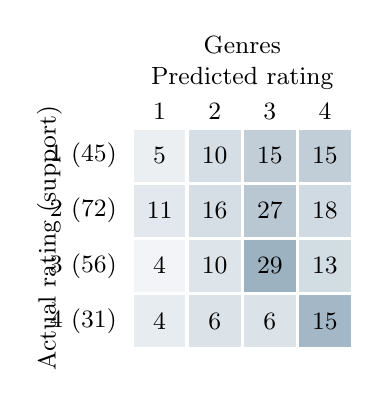
\begin{tikzpicture}[x=.70cm,y=.70cm,font=\small]
\node at (1.5,5) {Genres};\node at (1.5,4.4) {Predicted rating};\node at (0,3.8) {1};
\node at (1,3.8) {2};
\node at (2,3.8) {3};
\node at (3,3.8) {4};
\node[anchor=east] at (-.6,3) {1 (45)};
\fill[inkblue!9!white] (-0.47,2.5300000000000002) rectangle (0.47,3.4699999999999998);\node at (0,3) {5};
\fill[inkblue!19!white] (0.53,2.5300000000000002) rectangle (1.47,3.4699999999999998);\node at (1,3) {10};
\fill[inkblue!28!white] (1.53,2.5300000000000002) rectangle (2.4699999999999998,3.4699999999999998);\node at (2,3) {15};
\fill[inkblue!28!white] (2.5300000000000002,2.5300000000000002) rectangle (3.4699999999999998,3.4699999999999998);\node at (3,3) {15};
\node[anchor=east] at (-.6,2) {2 (72)};
\fill[inkblue!13!white] (-0.47,1.53) rectangle (0.47,2.4699999999999998);\node at (0,2) {11};
\fill[inkblue!19!white] (0.53,1.53) rectangle (1.47,2.4699999999999998);\node at (1,2) {16};
\fill[inkblue!32!white] (1.53,1.53) rectangle (2.4699999999999998,2.4699999999999998);\node at (2,2) {27};
\fill[inkblue!21!white] (2.5300000000000002,1.53) rectangle (3.4699999999999998,2.4699999999999998);\node at (3,2) {18};
\node[anchor=east] at (-.6,1) {3 (56)};
\fill[inkblue!6!white] (-0.47,0.53) rectangle (0.47,1.47);\node at (0,1) {4};
\fill[inkblue!15!white] (0.53,0.53) rectangle (1.47,1.47);\node at (1,1) {10};
\fill[inkblue!44!white] (1.53,0.53) rectangle (2.4699999999999998,1.47);\node at (2,1) {29};
\fill[inkblue!20!white] (2.5300000000000002,0.53) rectangle (3.4699999999999998,1.47);\node at (3,1) {13};
\node[anchor=east] at (-.6,0) {4 (31)};
\fill[inkblue!11!white] (-0.47,-0.47) rectangle (0.47,0.47);\node at (0,0) {4};
\fill[inkblue!16!white] (0.53,-0.47) rectangle (1.47,0.47);\node at (1,0) {6};
\fill[inkblue!16!white] (1.53,-0.47) rectangle (2.4699999999999998,0.47);\node at (2,0) {6};
\fill[inkblue!41!white] (2.5300000000000002,-0.47) rectangle (3.4699999999999998,0.47);\node at (3,0) {15};
\node[rotate=90] at (-2,1.5) {Actual rating (support)};
\end{tikzpicture}
\hspace{1cm}
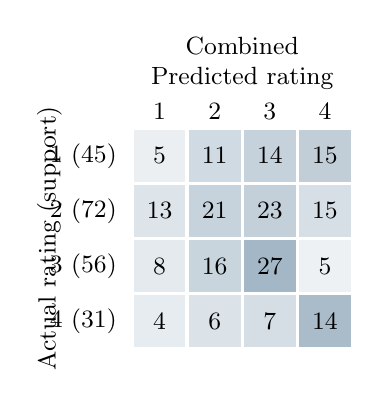
\begin{tikzpicture}[x=.70cm,y=.70cm,font=\small]
\node at (1.5,5) {Combined};\node at (1.5,4.4) {Predicted rating};\node at (0,3.8) {1};
\node at (1,3.8) {2};
\node at (2,3.8) {3};
\node at (3,3.8) {4};
\node[anchor=east] at (-.6,3) {1 (45)};
\fill[inkblue!9!white] (-0.47,2.5300000000000002) rectangle (0.47,3.4699999999999998);\node at (0,3) {5};
\fill[inkblue!21!white] (0.53,2.5300000000000002) rectangle (1.47,3.4699999999999998);\node at (1,3) {11};
\fill[inkblue!26!white] (1.53,2.5300000000000002) rectangle (2.4699999999999998,3.4699999999999998);\node at (2,3) {14};
\fill[inkblue!28!white] (2.5300000000000002,2.5300000000000002) rectangle (3.4699999999999998,3.4699999999999998);\node at (3,3) {15};
\node[anchor=east] at (-.6,2) {2 (72)};
\fill[inkblue!15!white] (-0.47,1.53) rectangle (0.47,2.4699999999999998);\node at (0,2) {13};
\fill[inkblue!25!white] (0.53,1.53) rectangle (1.47,2.4699999999999998);\node at (1,2) {21};
\fill[inkblue!27!white] (1.53,1.53) rectangle (2.4699999999999998,2.4699999999999998);\node at (2,2) {23};
\fill[inkblue!18!white] (2.5300000000000002,1.53) rectangle (3.4699999999999998,2.4699999999999998);\node at (3,2) {15};
\node[anchor=east] at (-.6,1) {3 (56)};
\fill[inkblue!12!white] (-0.47,0.53) rectangle (0.47,1.47);\node at (0,1) {8};
\fill[inkblue!24!white] (0.53,0.53) rectangle (1.47,1.47);\node at (1,1) {16};
\fill[inkblue!41!white] (1.53,0.53) rectangle (2.4699999999999998,1.47);\node at (2,1) {27};
\fill[inkblue!8!white] (2.5300000000000002,0.53) rectangle (3.4699999999999998,1.47);\node at (3,1) {5};
\node[anchor=east] at (-.6,0) {4 (31)};
\fill[inkblue!11!white] (-0.47,-0.47) rectangle (0.47,0.47);\node at (0,0) {4};
\fill[inkblue!16!white] (0.53,-0.47) rectangle (1.47,0.47);\node at (1,0) {6};
\fill[inkblue!19!white] (1.53,-0.47) rectangle (2.4699999999999998,0.47);\node at (2,0) {7};
\fill[inkblue!38!white] (2.5300000000000002,-0.47) rectangle (3.4699999999999998,0.47);\node at (3,0) {14};
\node[rotate=90] at (-2,1.5) {Actual rating (support)};
\end{tikzpicture}
\caption{Ordered confusion counts for the same 204 held-out titles (seed 156). Darker cells have larger within-row fractions. The diagonal is correct; opposite corners expose extreme rating errors.}\label{fig:confusions}\end{figure}

Both conditions make 19 extreme 1$\leftrightarrow$4 errors on this partition. Such mistakes matter for a viewing assistant even if a small mean BA gain exists. The notebook also reports paired corrections within every genre with at least 40 titles, including each rating's support; these overlapping subsets diagnose failures rather than provide independent studies.


\subsection{A Held-Out Prediction Explained}
I fixed \emph{The Great Dictator} from my opening example, rather than selecting a title the model happened to get right. The current held-out model predicts 
3 instead of my 4. Its outputs for ratings 1--4 are 19.10\%, 27.18\%, 30.18\%, 23.55\%. These are uncalibrated class-weighted outputs, not verified chances of my future enjoyment.

The score contrast decomposes into an intercept and feature contributions:
\[z_a-z_b=(b_a-b_b)+\sum_jx_j(w_{aj}-w_{bj}).\]

For predicted 3 versus true 4, a positive term favors 3. War contributes $+1.361$ because its normalized value 0.408 multiplies a coefficient difference of 3.335; Drama contributes $-0.703$. Summing all terms and the intercept gives $0.248$, also $\log(p_3/p_4)$. The ratio $e^{0.248}=1.28$ shows the model's relative preference between those two labels.

Only \emph{from, his, to, while} survive as nonzero text features in its 520-word training vocabulary. Distinctive details about satire and persecution do not contribute directly. This explains the mechanism of the error without asserting that common words caused my enjoyment; deleting a word would also change normalization.

\begin{figure}[htbp]\centering
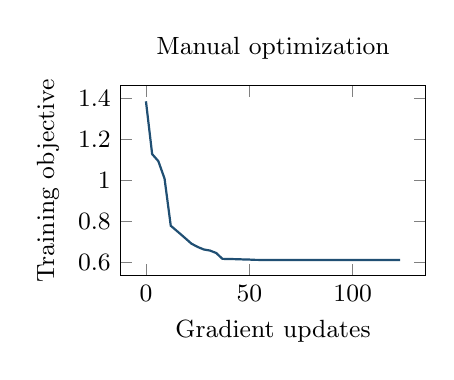
\begin{tikzpicture}
\begin{axis}[width=.45\linewidth,height=4cm,xlabel={Gradient updates},ylabel={Training objective},title={Manual optimization},font=\small]
\addplot[inkblue,thick] coordinates {(0,1.386294) (3,1.128036) (6,1.093276) (9,1.007953) (12,0.777408) (15,0.751477) (18,0.725431) (22,0.689795) (25,0.673680) (28,0.661165) (31,0.655926) (34,0.643851) (37,0.615364) (41,0.614415) (44,0.613745) (47,0.612572) (50,0.611802) (53,0.610320) (56,0.610225) (59,0.609881) (63,0.609875) (66,0.609859) (69,0.609854) (72,0.609834) (75,0.609824) (78,0.609807) (82,0.609805) (85,0.609804) (88,0.609796) (91,0.609792) (94,0.609792) (97,0.609792) (100,0.609792) (104,0.609792) (107,0.609792) (110,0.609792) (113,0.609792) (116,0.609792) (119,0.609792) (123,0.609792)};
\end{axis}\end{tikzpicture}
\hfill
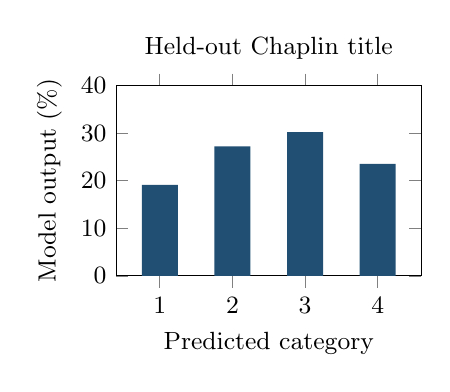
\begin{tikzpicture}
\begin{axis}[width=.45\linewidth,height=4cm,ybar,bar width=13pt,xmin=.4,xmax=4.6,ymin=0,ymax=40,xtick={1,2,3,4},xlabel={Predicted category},ylabel={Model output (\%)},title={Held-out Chaplin title},font=\small]
\addplot[fill=inkblue,draw=none] coordinates {(1,19.095658) (2,27.182158) (3,30.176348) (4,23.545835)};
\end{axis}\end{tikzpicture}
\caption{The optimization objective decreases, but the held-out title is still misclassified. Convergence checks the fitting calculation; it does not establish predictive usefulness.}\label{fig:worked}\end{figure}


\subsection{Learning Curves}
A separate diagnostic fixes $C=1$ and varies training size within the first repetition's outer folds. This holds the declared learning rule fixed rather than selecting another setting from outer scores. The plot compares how well the model fits its training titles with performance on titles it did not fit.

\begin{figure}[htbp]\centering
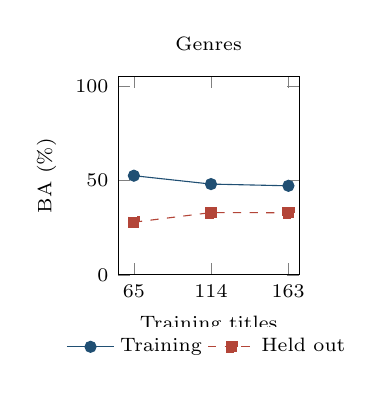
\begin{tikzpicture}
\begin{axis}[width=.32\linewidth,height=4.1cm,xmin=55,xmax=170,ymin=0,ymax=105,xtick={65,114,163},xlabel={Training titles},ylabel={BA (\%)},title={Genres},font=\scriptsize,legend style={at={(.5,-.26)},anchor=north,legend columns=2,draw=none,font=\scriptsize}]
\addplot[inkblue,mark=*] coordinates {(65.0,52.485162) (114.0,48.046327) (163.2,47.131784)};
\addplot[warmred,dashed,mark=square*] coordinates {(65.0,27.857143) (114.0,32.944805) (163.2,32.869048)};
\legend{Training,Held out}
\end{axis}\end{tikzpicture}
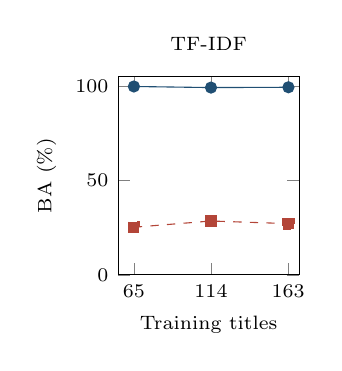
\begin{tikzpicture}
\begin{axis}[width=.32\linewidth,height=4.1cm,xmin=55,xmax=170,ymin=0,ymax=105,xtick={65,114,163},xlabel={Training titles},ylabel={BA (\%)},title={TF-IDF},font=\scriptsize,legend style={at={(.5,-.26)},anchor=north,legend columns=2,draw=none,font=\scriptsize}]
\addplot[inkblue,mark=*] coordinates {(65.0,99.722222) (114.0,99.143293) (163.2,99.307320)};
\addplot[warmred,dashed,mark=square*] coordinates {(65.0,25.186147) (114.0,28.496392) (163.2,27.105700)};

\end{axis}\end{tikzpicture}
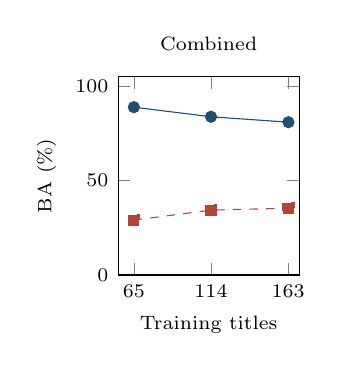
\begin{tikzpicture}
\begin{axis}[width=.32\linewidth,height=4.1cm,xmin=55,xmax=170,ymin=0,ymax=105,xtick={65,114,163},xlabel={Training titles},ylabel={BA (\%)},title={Combined},font=\scriptsize,legend style={at={(.5,-.26)},anchor=north,legend columns=2,draw=none,font=\scriptsize}]
\addplot[inkblue,mark=*] coordinates {(65.0,88.880607) (114.0,83.806877) (163.2,80.922830)};
\addplot[warmred,dashed,mark=square*] coordinates {(65.0,29.061328) (114.0,34.371934) (163.2,35.398629)};

\end{axis}\end{tikzpicture}
\caption{Mean fold scores at approximately 65/114/163 training titles. Blue is training; dashed red is held out. Subsets and folds overlap; no independent uncertainty interval is implied.}\label{fig:curves}\end{figure}

At the largest size, text training BA is 99.31\% while held-out BA is 27.11\%; combined is 80.92\% versus 35.40\%. That gap is consistent with fitting word associations that transfer poorly. It does not identify a single cause or guarantee more ratings will repair it. The smaller subsets are stratified but not nested; vocabulary, sample composition and class weights change, and fixed $C$ changes effective shrinkage as $S$ changes. These curves diagnose the whole procedure rather than isolate sample count alone.


\subsection{Related Works and LDA}

The conservative map has 146 groups, with 31 multi-title families. Grouped nested CV scores 31.86\% for genres and 29.80\% combined (-2.06 pp). Keeping related titles apart therefore does not preserve a text advantage in this run. The map leaves broader shared-universe ties unresolved, and changed folds alter the prediction target; this result is sensitivity evidence, not a precise estimate of leakage.


LDA offers a different compression of the synopsis. It imagines choosing a hidden topic from the description's mixture $\theta_d$, then drawing a word from that topic's word distribution $\beta_j$:
\[
P(w=t\mid d)=\sum_{j=1}^{5}\theta_{dj}\beta_{jt}.
\]
The sum accounts for five possible hidden routes to the word. Training infers topic mixtures and word distributions that make the training text plausible, without seeing liking labels. Both distributions are nonnegative and sum to one. Symmetric Dirichlet priors with entries $1/5$ favor concentrated mixtures when evidence is scarce; they supply a fixed preference over proportions rather than additional observations. Twenty batch iterations approximate the fit. Word counts match this occurrence model; the five inferred topic proportions then feed the same logistic classifier \cite{blei,topics}.

The five-topic procedure was fixed before this rerun, with topics learned inside each training fold and the same three $C$ choices. Topics alone score 22.87\%; genres plus topics score 32.81\%, versus 33.38\% for genres on the same partitions. This bounded topic representation does not add useful evidence here. It does not establish universal TF-IDF superiority: topic compression may discard a detail that distinguishes my taste, and different preprocessing is involved. Short descriptions supply limited co-occurrence evidence; neither visually coherent topics nor human topic names prove preference prediction.


\FloatBarrier
\section{Discussion and Next Steps}

My answer is conditional. With a fixed logistic learning rule, descriptions add only +0.53 pp on average and the sign changes across partitions. The development-selected CV family procedures add +2.13 pp on their three smaller common tests, but use different selected families and overlapping titles; the grouped check reverses the text contrast. Together these findings leave substantial uncertainty about a dependable improvement beyond genres. A favorable mean alone is insufficient to trust the system to choose my evening's viewing.


The archive reflects my saved-list habits, platform access, what I chose to watch, recall and partial (but substantial) viewing. It cannot represent unselected streaming titles or other viewers. A series rating compresses far more exposure than a movie rating. 130 zero-rated titles have unknown preferences, not low liking. The 90 anonymous Netflix events leave unknown coverage gaps. Short synopses omit acting, pacing, visual style and viewing context. I also didn't measure my present mood, so my semester's goal remains a future target.

The next useful step is to collect more independent ratings with stable category anchors and notes on the desired mood and whether the title delivered it. I also want to test longer plot summaries and explicit adaptation information, such as whether a title is based on a book, because short blurbs may omit signals relevant to my taste.

Alongside ordinal prediction, I will compare TF-IDF with embeddings from a pretrained neural network: numerical text representations intended to place similar meanings close together. These could support semantic searches for a desired mood and serve as classifier inputs. I would compare short and longer descriptions using the same representation first, then compare representations on the same text, so any gain can be traced to more complete information or a different way of representing it. A newly fixed evaluation plan would test whether these changes improve held-out classification, rather than assuming that longer text or a neural model must help.

\textbf{Reproducibility.} The current notebook contains source-to-title replay, Excel-to-CSV label import, loss/gradient/update code, numerical reference checks, frozen splits, selected parameters, held-out predictions and all plotted outputs.

\textbf{GitHub Link to Code}: \href{https://github.com/JamesOlaitan/CS156-ML-Repo}{https://github.com/JamesOlaitan/CS156-ML-Repo}

\clearpage
\begin{thebibliography}{99}\small
\bibitem{netflix} Netflix. \href{https://help.netflix.com/en/node/101917}{Viewing history and device activity}.
\bibitem{imdblists} IMDb. \href{https://help.imdb.com/article/imdb/track-movies-tv/faq-for-the-list-feature/GNQMN47VZSE7KW38}{Lists FAQ}. Source snapshots acquired October 17, 2026.
\bibitem{sklearntext} scikit-learn. \href{https://scikit-learn.org/stable/modules/feature_extraction.html#tfidf-term-weighting}{TF-IDF feature extraction}.
\bibitem{course} CS156, Fall 2026. \href{https://forum.minerva.edu/app/courses/4077/sections/13536/classes/104897}{Session 6: likelihood and gradients}; \href{https://forum.minerva.edu/app/courses/4077/sections/13536/classes/104899}{Session 7: perceptron learning}; \href{https://forum.minerva.edu/app/courses/4077/sections/13536/classes/105072}{Session 8: gradients}; \href{https://forum.minerva.edu/app/courses/4077/sections/13536/classes/105074}{Session 9: validation}.
\bibitem{svm} scikit-learn. \href{https://scikit-learn.org/stable/modules/generated/sklearn.svm.LinearSVC.html}{LinearSVC: squared-hinge loss and multiclass handling}.
\bibitem{cnb} scikit-learn. \href{https://scikit-learn.org/stable/modules/naive_bayes.html#complement-naive-bayes}{Complement Naive Bayes: complement statistics and smoothing}.
\bibitem{tree} scikit-learn. \href{https://scikit-learn.org/stable/modules/tree.html#mathematical-formulation}{Decision trees: impurity, weighting and complexity}.
\bibitem{nested} scikit-learn. \href{https://scikit-learn.org/stable/auto_examples/model_selection/plot_nested_cross_validation_iris.html}{Nested versus non-nested cross-validation}.
\bibitem{bates} S. Bates, T. Hastie, R. Tibshirani. \href{https://arxiv.org/abs/2104.00673}{Cross-validation: what does it estimate and how well does it do it?} 2021.
\bibitem{blei} D. Blei, A. Ng, M. Jordan. \href{https://www.jmlr.org/papers/volume3/blei03a/blei03a.pdf}{Latent Dirichlet Allocation}. \emph{JMLR} 3:993--1022, 2003.
\bibitem{topics} scikit-learn. \href{https://scikit-learn.org/stable/auto_examples/applications/plot_topics_extraction_with_nmf_lda.html}{Count-based topic extraction}.
\end{thebibliography}
\end{document}
